\subsection{Sparx Systems Enterprise Architect}
\def \entArch {\textsf{Enterprise Architect}}
Sparx Systems \entArch\ is another tool that provides modeling of UML diagrams.
It supports mind map diagrams and project management, to provide full traceability from requirements specification to deployment end implementation.
This tool also provides also some metrics evaluation to compute the complexity of a project only based on Use Case diagrams. 

To perform this evaluation, the user needs to provide a level of implementation complexity to each interaction with authors. 
This task can be done when defining the Use Case descriptions or when performing the metrics evaluation.

To evaluate the metrics, \entArch\ have a wizard, that gives also other options to do the complexity analysis.
This options manipulates the Technical complexity and also Environment complexity and be used to adapt the evaluation and perform a better result on estimation.

Also can be filtered the Use Cases used in evaluation. 
To filter can be used manual selection or regular expressions over use case name.
This kind of filtering ables the project to be distributed and evaluated individually.

The final result presented is the maximum number of working hours needed to perform the implementation.

\subsubsection{Results}

To use this tool in metrics calculation, have the possibility do some tweaking over use case complexity, on their description, to get more precise results. This complexity admits simple values like low, medium or high for complexity.
We could also edit some related factors related to environment complexity, technics complexity or hour rates in the wizard shown on the left side of figure \ref{img:sparxRes}. Here we can use multiple factors to evaluate this factors, like usability or portability on technical complexity.
At the end we open the Use Case metrics wizard and it is presented to us, as in the right side in figure \ref{img:sparxRes}, the set of default values used to evaluate the effort of task.

\begin{figure}[h]
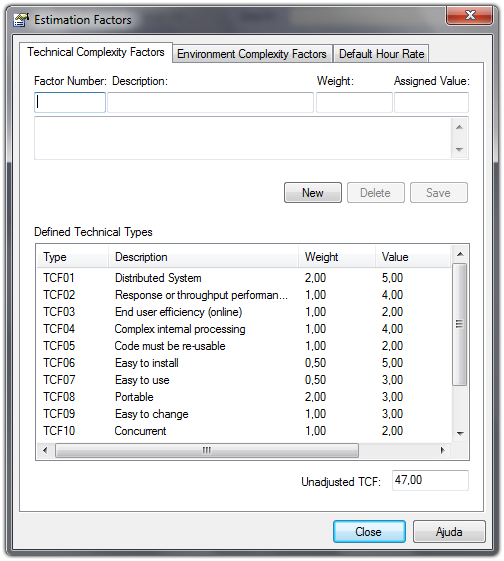
\includegraphics[scale=0.257]{images/sparxestim.png}
\hspace{0.1cm}
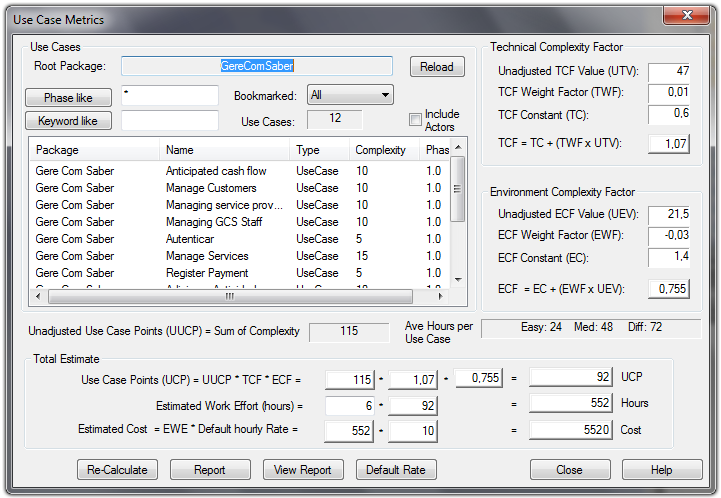
\includegraphics[scale=0.29]{images/sparx.png}
\caption{Estimation Factors and Use Case Metrics \entArch\ wizards}\label{img:sparxRes}
\end{figure}

The final results of metrics evaluation with this tool, is an estimation of Working Hours, Use Case Points\cite{Ribu01estimatingobject-oriented} and Total Cost needed to perform the development of modeled system.

In Our case, because we have twelve Use Cases and had many of them with medium complexity. The effort to complete the task is 552 working hours, that would give a final result of \EUR{5.520}. To obtain this value only was changed the use cases complexity and everything else was left with default values.
